\documentclass[twocolumn,11pt]{IEEEtran}
\usepackage[verbose,expansion=alltext,stretch=50]{microtype}
\usepackage{graphicx}

\title{Optimizing Scheduling Policies For Heterogeneous Distributed Systems}

\author{
   
   \begin{tabular}{c| c| c| c}
       Mohamed Shawky & Remonda Talaat & Mahmoud Adas & Evram Youssef\\
       \texttt{\small{SEC 2, B.N 16}} & \texttt{\small{SEC 1, B.N 20}} & \texttt{\small{SEC 2, B.N 21}} & \texttt{\small{SEC 1, B.N 9}}
   \end{tabular}%
   
   \texttt{\small{\{mohamedshawky911, remondatalaat21, mido3ds, evramyousef\}@gmail.com}}
}%

\markboth{Cairo Uni. CMP Dep. | OS Research | Phase 3 | Team 10 | \today}{Shell}

\begin{document}
    \maketitle

    \begin{abstract}
        This is the second report of the research project.
        This report discusses our methodology for the proposed problem and our potential experiments.
    \end{abstract}

    \section{Introduction}
    \IEEEPARstart{T}{he} scheduling and resource allocation policies for a distributed system are very hard to achieve. This becomes even harder when the system is heterogeneous, where you have different types of chips. The problem is classified as \emph{NP Hard} and it's an open problem for research. Recursive optimization is one practical solution to reach a sub-optimal or even an optimal policy. In this work we will discuss several possible solutions to the problem and introduce yet a new idea that could potentially work better.
    
    \section{Formulation}
    To simulate the real heterogeneous systems, we have to create a simulation stub, where you have some defined machines with their specifications and a list of jobs that need to be executed on such machines. We will work with \emph{Global Static} scheduling scheme and the goal is to assign the jobs to the machines at each time step to maximize overall performance. Although resource utilization isn't our main concern, we may include it in our objective.
    
    \section{Methodology}
    
    \subsection{Baseline}
    First, let's discuss the baseline that all other experiments will be compare with. \emph{Heterogeneous Earliest Finish Time (HEFT)} will be considered as our baseline. \emph{(HEFT)} is an old well-established algorithm for scheduling in heterogeneous systems. Basically, the algorithm schedules a job on a machine based on job requirements with its earliest finish time. Although it's very simple, it's used as a comparison baseline for most of the research work made on this problem.  
    
    \subsection{Genetic Algorithms}
    Our first attempt with recursive optimization for scheduling will be genetic algorithms. Genetic algorithms have proven to be very efficient in solving some of the hardest optimization problem. Previous work has been done in using genetic algorithms to solve scheduling problems. We will attempt using genetic algorithms to solve our proposed problem. The targeted \emph{fitness function} will be the average waiting time for all jobs. 

    \subsection{Reinforcement Learning}
    Another possible solution is \emph{Reinforcement Learning (RL)}, which is one on the most dominant fields in optimization and decision making problems. The main advantage of \emph{RL} is that it can act in a very dynamic environment, so it can adapt to priority changes and deadlocks, for instance. Moreover, we can add extra layers of complexity to our problem, such as: adding a status to each machine which can change with time or machine-specific task which needs to be executed on a specific machine. However, this comes at a cost of complicated and unstable environment. \\
    If RL is to be used, one can consider using \emph{Q-Learning} to learn a scheduling policy using an environment of some machines. 

    \subsection{Neural Networks (Deep Learning)}
    The main novel idea of this work will be the usage of \emph{neural networks} for the scheduling problem. \emph{Neural Networks} are known to be very good at learning representations and function approximation. In this work, we propose an architecture that can be used to reach a good approximated solution for the scheduling problem.\\
    Previous work tried to use \emph{neural networks} to solve scheduling problem through \emph{Hopfield Nets} and \emph{Inhibitor Neurons}. However, we will try to make use of the recent advances in \emph{Deep Learning} to redefine the scheduling problem and solve it.
    
    \subsubsection{Architecture}
    Our architecture consists of two encoders and one decoder, as shown in Fig.\ref{fig:nn}. \\
    The first encoder is a simple feedforward fully connected network, to which is machines specifications are passed. This encoder learns a representation for the machines to be able to use it later in producing the outputs. \\
    The second encoder is an \emph{Recurrent Neural Network (RNN)}, to which the jobs are passed one by one ordered by the arrival time. This network learns a representation of the jobs preserving the arrival order. \\
    The representation of the jobs is later passed to an RNN decoder, which produces \emph{N} timesteps, at each step the processes currently running on each machine. The output is supported by attention modules to be able to take the machines representation into account when distributing the jobs.
    
    \begin{figure}[hp]
        \centering
        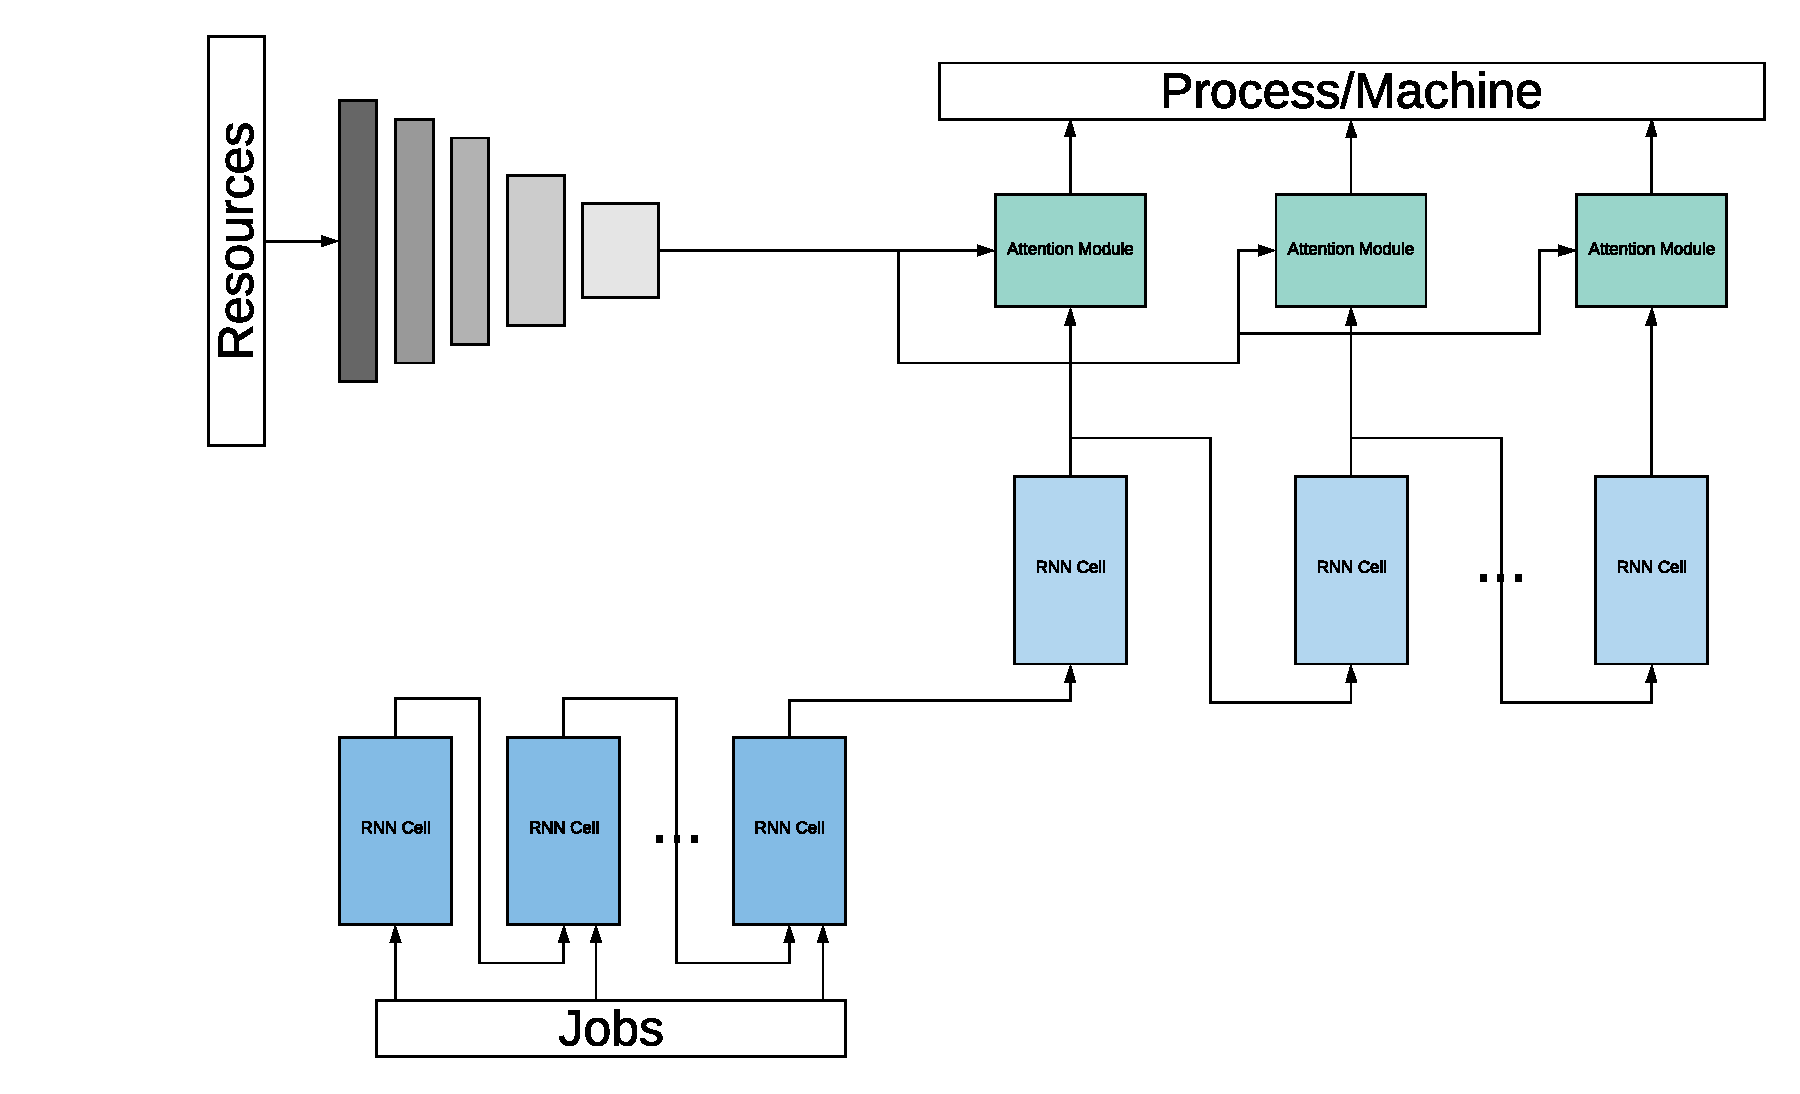
\includegraphics[width=0.45\textwidth]{sched_nn}
        \caption{The architecture of the proposed neural network for Heterogeneous systems scheduling}
        \label{fig:nn}
    \end{figure}
    
    \subsubsection{Objective Function}
    The cost function defined for this problem will be a simple \emph{mean square error (MSE)} between the output \emph{(processes/machine)} and some optimally solved examples.
    
    \subsubsection{Downsides}
    The main downside of the proposed solution is that we have to know the maximum number of machines and the maximum number of jobs to be able to define the network. However, the network scheduling inference can be faster than many algorithms. 
    
    \section{Experiments}
    This work will many focus of performance, specifically average waiting time and average turnaround time. 
    \begin{itemize}
        \item Measure the performance of \emph{HEFT} on our simulation stub.
        \item Experiment with Genetic Algorithms to explore possible improvements.
        \item Try the proposed neural network and explore the results and possible improvements.
        \item Experiment with \emph{RL} on our simulation stub. \emph{[OPTIONAL]}
    \end{itemize}
    
    \section{References}
    \subsection*{[1] Kumar, Ranjeet \& Dr.Rakesh, \& Er.Rajiv, \& Gill, Er \& Kaushik, Ashwani. (2010). Genetic Algorithm approach to Operating system process scheduling problem. International Journal of Engineering Science and Technology.}
    \begin{itemize}
        \item Why this paper: To explore the formulation of a scheduling problem using \emph{Genetic Algorithms}.
        \item Paper research problem: Operating systems process scheduling.
        \item Paper goal: To improve scheduling with \emph{Genetic Algorithms}.
        \item Conclusion: \emph{Genetic Algorithms} has a potential in such problems.
    \end{itemize} 
    
     \subsection*{[2] Alexandru Iulian Orhean, Florin Pop, Ioan Raicu,
    New scheduling approach using reinforcement learning for heterogeneous distributed systems,
    Journal of Parallel and Distributed Computing.}
    \begin{itemize}
        \item Why this paper: To understand the scheduling problem as an \emph{RL} model.
        \item Paper research problem: \emph{RL} modelling for scheduling.
        \item Paper goal: Explore all layers of complexity of a scheduling problem using \emph{RL}.
        \item Conclusion: \emph{RL} can be very useful in dynamic scheduling.
    \end{itemize} 
    
    \subsection*{[3] Chillet, Daniel \& Eiche, Antoine \& Pillement, Sébastien \& Sentieys, Olivier. (2011). Real-time scheduling on heterogeneous system-on-chip architectures using an optimised artificial neural network. Journal of Systems Architecture - Embedded Systems Design. 57. 340-353. 10.1016/j.sysarc.2011.01.004.}
    \begin{itemize}
        \item Why this paper: To explore the previous work made about the usage of neural networks in scheduling tasks.
        \item Paper research problem: Process scheduling with \emph{ANNs}.
        \item Paper goal: To improve the usage of neural networks in scheduling.
        \item Conclusion: Neural networks can be a good candidate for scheduling.
    \end{itemize} 

\end{document}


